\subsection{LENS exceeded OneNet under both measurement designs in two systems}
\label{sec:measurement-placement}

Both distributed and restricted LENS achieved higher mean AUPRC than OneNet in Carlstr\"om and Sch\"afer at the largest evaluated budgets (Figure~\ref{fig:measurement-placement}).
These comparisons used equal numbers of training labels and identical test pairs, as described in Section~\ref{sec:measurement-placement-methods}.
Distributed measurements gave higher mean performance than restricted measurements at these budgets, although the advantage varied across partitions and was less consistent in Carlstr\"om.
The results suggest that broader measurement coverage can help, while supporting restricted measurements as a useful option in some systems.

\begin{figure}[!t]
\centering
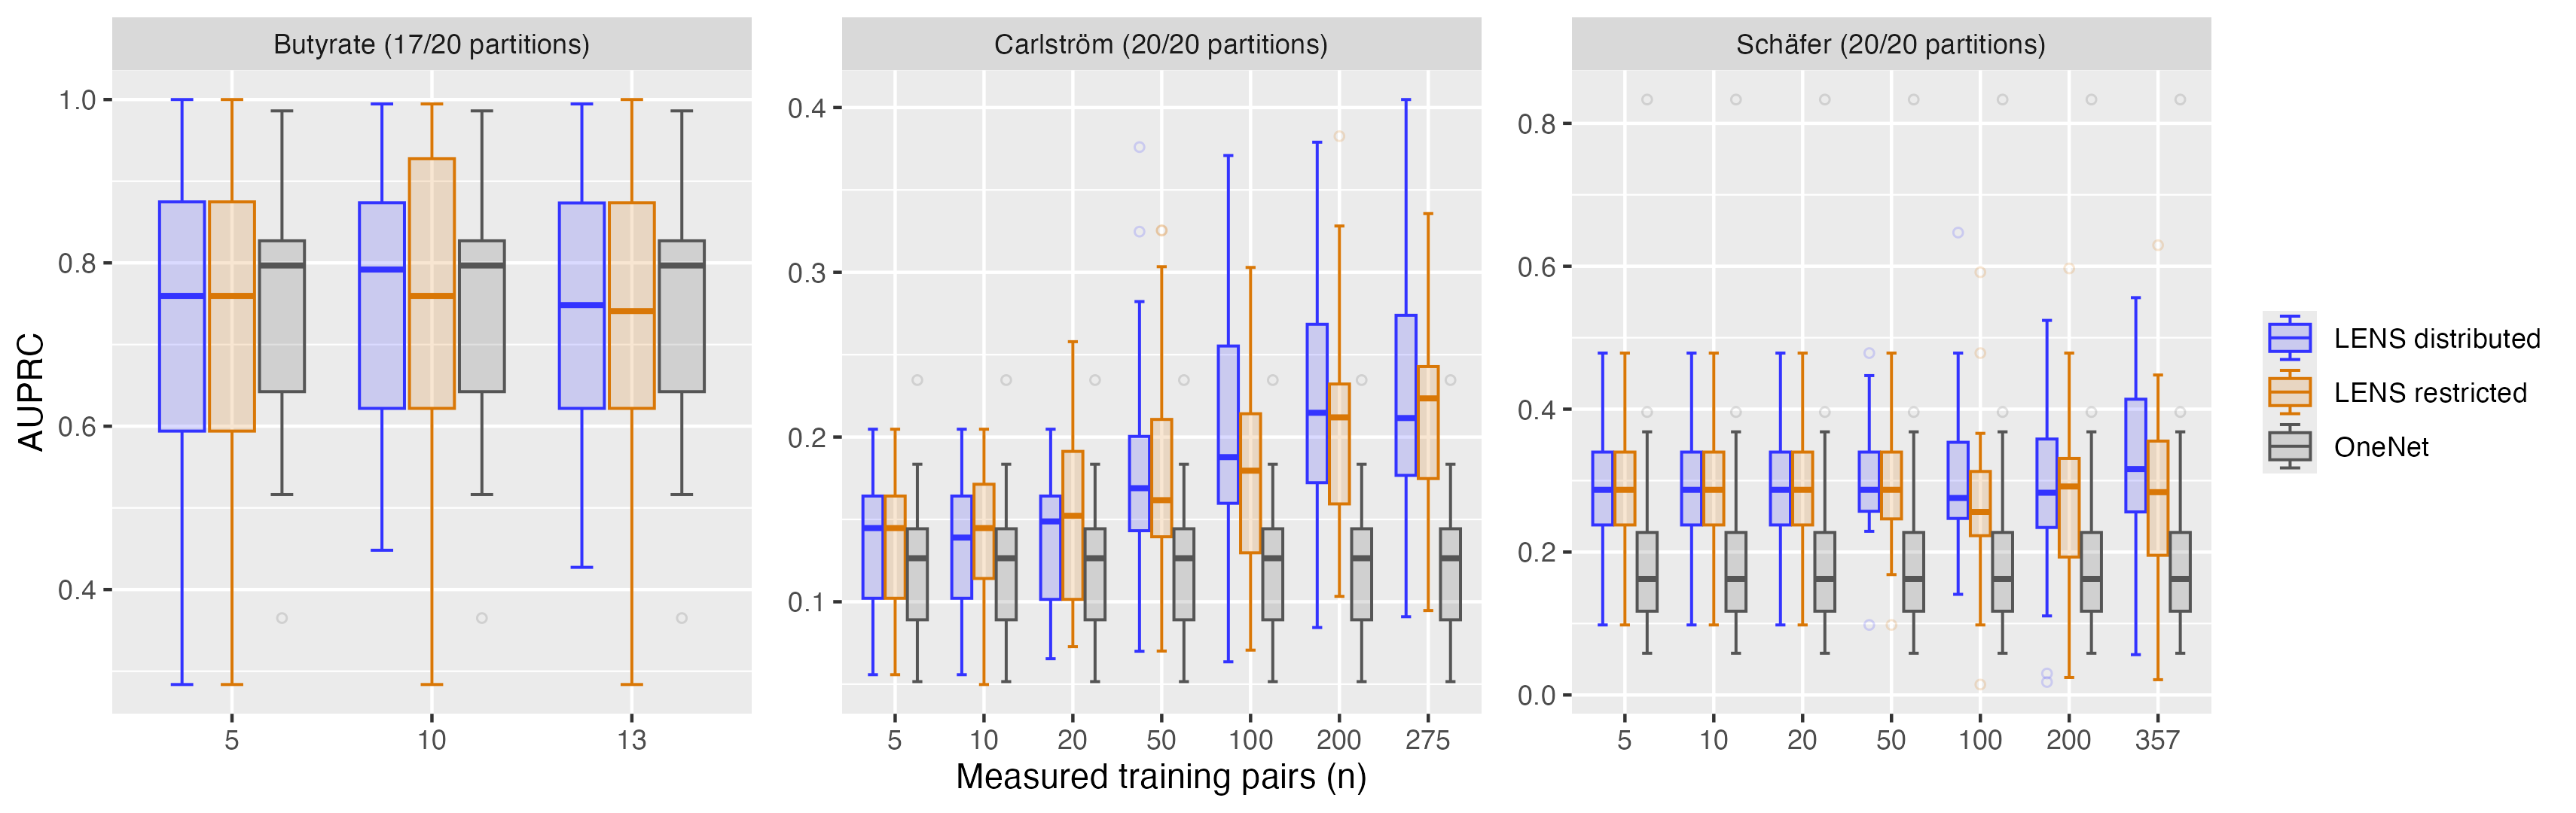
\includegraphics[width=\textwidth]{measurement_placement.png}
\caption{AUPRC of LENS under distributed and restricted measurement designs, compared with OneNet.}
\label{fig:measurement-placement}
\end{figure}

In Carlstr\"om, both measurement designs exceeded OneNet in every partition at the maximum training budget.
Restricted LENS therefore provided useful rankings relative to OneNet even when neither taxon in a test pair had measured interactions available for training.
In Sch\"afer, both designs also exceeded OneNet on average, with higher mean performance under distributed measurements.
This pattern supports broader measurement coverage as a promising option, although the variation across partitions prevents a general recommendation that distributed measurements will always perform better.

Neither design exceeded OneNet on average in Butyrate at the maximum budget.
The restricted training pool limited the comparison to 13 measured pairs.
This shortage of training labels, together with the limited test coverage, may explain the absence of an advantage over OneNet; it does not establish that the number of abundance samples was responsible.
OneNet may also already capture useful ranking information in this system.
